\documentclass[a4paper,fleqn]{cas-dc}

\usepackage[T1]{fontenc}
\usepackage{graphicx}
\usepackage{booktabs}
\usepackage{multirow}
\usepackage{amsmath}
\usepackage{array}
\usepackage{microtype}
\usepackage{enumitem}
\usepackage{placeins}
\usepackage{url}

\sloppy
\emergencystretch=2em
\setlength{\tabcolsep}{5pt}

\begin{document}
\let\WriteBookmarks\relax
\shorttitle{PlantDiseaseNet-Hybrid}
\title[mode=title]{A Hybrid Deep Learning Framework for Multi-Crop Plant Disease Classification Using Strategic Data Augmentation}
\author[1]{Author Name}
\ead{author@iiitp.ac.in}
\author[1]{Anupama Arun}
\ead{anupamaarun21@cse.iiitp.ac.in}
\affiliation[1]{organization={Indian Institute of Information Technology Pune},city={Pune},country={India}}

\begin{abstract}
Automated plant disease recognition is attractive for large-scale crop monitoring, but performance reported on controlled leaf-image datasets does not by itself establish robustness across crops, disease morphologies, or changes in image appearance. This study presents PlantDiseaseNet-Hybrid, a compact hybrid convolutional architecture that combines two deliberately different feature-fusion mechanisms. Parallel $3\times3$, $5\times5$, and $7\times7$ convolutions form multi-scale responses which are fused by element-wise addition, keeping the channel width fixed within each Inception cell. Later $7\times7$ convolutional features are combined with their input through channel-wise concatenation, preserving earlier representations for downstream processing. The design therefore uses additive fusion where redundant channel expansion is undesirable and concatenative fusion where feature preservation and reuse are desirable.

The study is organized as a sequence of controlled experiments rather than a single aggregate benchmark. The proposed architecture is evaluated separately on wheat, cotton, and PlantVillage subsets and on a combined 24-class setting. Architecture-level ablations replace the hybrid connectivity with standard Inception, residual addition, Inception-only addition, or skip concatenation. A separate augmentation study is retained as an independent experimental section so that the effect of image transformations is not conflated with the architectural contribution. Soybean experiments are reported separately because their dataset and experimental protocol constitute a distinct evaluation setting. The executed repository evidence currently verifies accuracies of 97.81\% on wheat, 53.55\% on cotton, 97.67\% on PlantVillage, and 95.91\% for the combined proposed model. The architecture ablations obtain 95.33\%, 96.04\%, 95.84\%, and 95.67\% for standard Inception, ResNet-style residual learning, Inception with additive fusion, and skip concatenation, respectively. These results indicate that the benefit of the proposed design should be interpreted in relation to crop composition and the complementary roles of its two fusion operations. The augmentation and soybean sections are retained as independent studies and are only populated with numerical claims where executed notebook outputs provide direct evidence.
\end{abstract}

\begin{keywords}
plant disease classification \sep hybrid CNN \sep Inception \sep feature fusion \sep skip connections \sep data augmentation \sep agricultural computer vision
\end{keywords}
\maketitle

\section{Introduction}
Plant disease recognition is a recurring problem in precision agriculture because visible symptoms can appear as small changes in colour, texture, lesion geometry, venation, or leaf structure. Manual inspection remains valuable, but it is labour-intensive and depends on specialist judgement. Image-based learning offers a complementary route in which disease-related visual patterns can be learned directly from labelled examples. The feasibility of this approach was demonstrated on PlantVillage by Mohanty et al., who trained deep convolutional models on tens of thousands of controlled leaf images \cite{mohanty2016}.

The success of deep CNNs, however, creates a second problem: increasingly large networks can improve representation capacity at the cost of memory, computation, and reduced transparency about which architectural mechanism is responsible for an observed gain. Inception introduced parallel multi-scale processing as a way of improving the use of computation \cite{szegedy2015}. ResNet subsequently showed that explicit residual pathways can make deep optimization easier \cite{he2016}. DenseNet demonstrated another form of connectivity in which earlier feature maps are retained and reused through concatenation \cite{huang2017}. These ideas are useful for plant disease recognition because symptoms occur at multiple spatial scales, while fine-grained discrimination can depend on retaining low- and mid-level evidence.

The present work asks a more specific architectural question: can the two fusion behaviours be used selectively in one compact model? The proposed PlantDiseaseNet-Hybrid uses additive fusion inside its Inception cells and concatenative fusion in its skip blocks. Addition keeps the output channel count equal to the requested filter count, avoiding the immediate channel multiplication that would follow branch concatenation. Concatenation is then used later, where retaining the original representation alongside newly transformed features is considered more valuable than forcing those representations into one tensor by addition. The design is therefore not a claim that addition is universally superior to concatenation, or vice versa. Rather, the hypothesis is that the two operations serve different representational purposes and can be assigned to different stages of the network.

A second objective is to separate architectural evaluation from data augmentation. Augmentation changes the training distribution and can alter generalization independently of the network design. Consequently, the augmentation experiments are treated as a dedicated study rather than being folded into the primary architectural comparison. This organization follows the general experimental logic used in recent plant-disease work where original and augmented training conditions are explicitly compared; Mhala et al., for example, reported separate original and augmentation/regularization conditions for potato disease classification \cite{mhala2025}.

The main contributions are:
\begin{itemize}[leftmargin=*]
\item a hybrid CNN in which multi-scale Inception responses are fused by element-wise addition;
\item concatenation-based skip connectivity that preserves the preceding representation for feature reuse;
\item a crop-wise and combined-dataset evaluation that exposes differences between individual datasets rather than hiding them behind one pooled score;
\item architecture ablations that isolate the contribution of the principal fusion mechanisms;
\item a separate augmentation study and a separate soybean study, preventing changes in data distribution from being presented as architectural evidence.
\end{itemize}

\section{Related Work}
\subsection{Deep learning for plant disease recognition}
PlantVillage established an important benchmark for image-based disease recognition, with a large collection of labelled plant leaf images and a deep-learning evaluation demonstrating high performance under controlled imaging conditions \cite{mohanty2016}. Subsequent studies have explored lightweight CNNs, transfer learning, attention mechanisms, explainable models, and field-acquired datasets. The literature increasingly emphasizes that controlled-dataset accuracy and field robustness are not interchangeable outcomes.

\subsection{Multi-scale representation and feature connectivity}
Inception-style networks process an input through parallel filters of different receptive-field sizes \cite{szegedy2015}. This is particularly relevant to leaf disease recognition because symptoms may range from fine texture changes to larger lesion structures. ResNet instead introduces residual addition, learning a residual transformation relative to the input \cite{he2016}. DenseNet uses concatenation to retain features from earlier layers and promote feature reuse \cite{huang2017}. The present architecture combines the design motivations of these approaches without reproducing any one of them directly.

\subsection{Augmentation as an experimental variable}
Augmentation is not merely a preprocessing convenience. It changes the range of appearances presented during optimization and can be especially useful when datasets contain imbalance or limited visual diversity. Mhala et al. studied original and augmented conditions alongside regularization for real-world potato disease images and reported measurable changes in performance under those conditions \cite{mhala2025}. In the present study, augmentation is therefore reported as a distinct experimental axis. No numerical improvement is attributed to augmentation unless the corresponding executed experiment provides a directly verifiable result.

\section{Materials and Methods}
\subsection{Datasets}
The repository contains experiments on wheat disease images, cotton disease images, PlantVillage subsets, a combined multi-crop collection, and a separate soybean study. The primary non-augmented experiments use three crop-specific notebooks: NB1 for wheat, NB2 for cotton, and NB3 for PlantVillage. The combined experiments use the same proposed hybrid design and compare it with architecture variants.

The PlantVillage component is grounded in the public PlantVillage resource described by Mohanty et al. \cite{mohanty2016}. The soybean experiments are kept separate because the repository associates them with the Auburn Soybean Disease Image Dataset (ASDID), an independently published dataset containing eight soybean disease/deficiency categories and healthy leaves \cite{bevers2022}. The official ASDID archive is maintained through Dryad \cite{dryad2022}.

For dataset reporting, the manuscript distinguishes the source dataset from the local experimental subset. This distinction is important because the number of classes in a particular experiment need not equal the number of classes in the full public dataset.

\begin{table*}[t]
\centering
\caption{Primary executed experiments retained for the manuscript. Values are taken from executed notebook outputs or repository result logs; no unverified metrics are substituted.}
\label{tab:primary}
\begin{tabular}{p{2.0cm}p{3.0cm}p{1.1cm}p{5.0cm}p{1.6cm}}
\toprule
Experiment & Dataset & Classes & Model / purpose & Accuracy (\%)\\
\midrule
NB1 & Wheat Disease & 3 & PlantDiseaseNet-Hybrid; crop-specific evaluation & 97.81\\
NB2 & Cotton Disease & 6 & PlantDiseaseNet-Hybrid; crop-specific evaluation & 53.55\\
NB3 & PlantVillage & 15 & PlantDiseaseNet-Hybrid; crop-specific evaluation & 97.67\\
Primary combined & Combined multi-crop & 24 & PlantDiseaseNet-Hybrid; proposed architecture & 95.91\\
\bottomrule
\end{tabular}
\end{table*}

\subsection{Image preprocessing}
All images used by the proposed architecture are resized to $256\times256$ pixels and represented as three-channel RGB inputs. Pixel normalization is applied before optimization. The preprocessing stage is intentionally separated from the augmentation study: resizing and normalization establish a common numerical representation, whereas augmentation changes the visual distribution presented to the model.

\begin{figure*}[t]
\centering
\IfFileExists{paper_figures/preprocessing_pipeline.png}{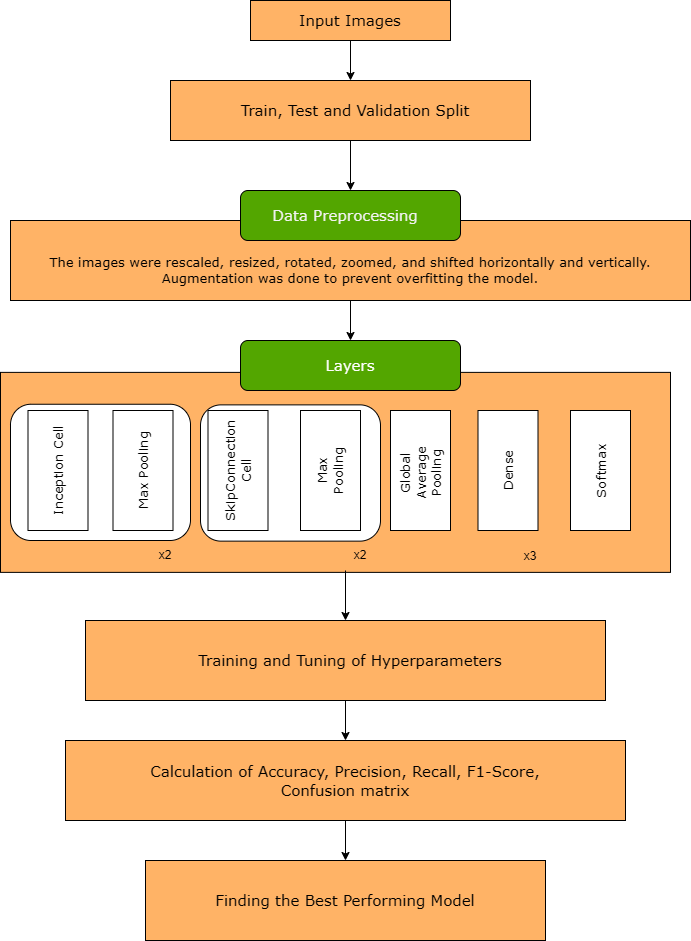
\includegraphics[width=0.90\textwidth,height=0.72\textheight,keepaspectratio]{paper_figures/preprocessing_pipeline.png}}{}
\caption{Preprocessing and augmentation workflow.}
\label{fig:preprocessing}
\end{figure*}

\subsection{Data augmentation study}
The augmentation study considers geometric and appearance transformations used in the repository, including horizontal flipping, rotation, zoom, brightness adjustment, translation, and contrast modification. These transformations target different sources of visual variability: orientation changes, scale changes, illumination changes, spatial displacement, and appearance variation.

The augmentation study is reported separately from the primary model results for two reasons. First, augmentation changes the effective training distribution and therefore cannot be treated as an architectural constant. Second, the repository contains several augmentation notebooks with different experimental configurations. Some are executed training studies without a directly verifiable final test metric in the stored notebook output. Such runs are retained in the repository as experimental records but are not converted into unsupported numerical claims in this manuscript.

\begin{table}[t]
\centering
\caption{Augmentation transformations considered in the study.}
\label{tab:augmentation}
\begin{tabular}{p{2.2cm}p{4.4cm}}
\toprule
Transformation & Intended variability represented\\
\midrule
Horizontal flip & Leaf orientation and camera viewpoint\\
Rotation & Non-canonical leaf orientation\\
Zoom & Scale and framing variation\\
Brightness & Illumination changes\\
Translation & Off-centre positioning\\
Contrast & Appearance and illumination variation\\
\bottomrule
\end{tabular}
\end{table}

\subsection{PlantDiseaseNet-Hybrid architecture}
The network receives a $256\times256\times3$ RGB image. Two Inception cells are followed by two skip-connection blocks, four max-pooling stages, global average pooling, and fully connected classification layers. The implementation uses 16 filters in the first Inception cell, 32 in the second, 64 new filters in the first skip block, and 128 new filters in the second skip block. Because the skip blocks concatenate the transformed representation with their input, the channel dimensions increase from 32 to 96 and from 96 to 224, respectively.

\begin{figure*}[t]
\centering
\IfFileExists{paper_figures/overall_architecture.png}{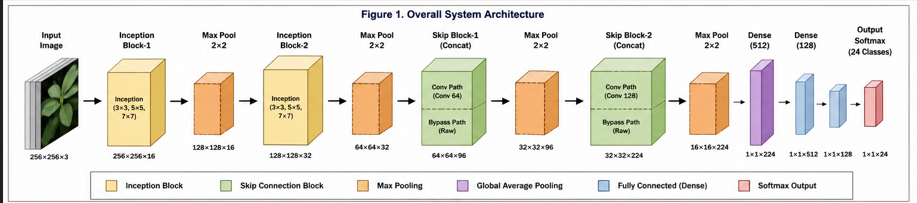
\includegraphics[width=0.94\textwidth,height=0.70\textheight,keepaspectratio]{paper_figures/overall_architecture.png}}{}
\caption{Overall PlantDiseaseNet-Hybrid architecture.}
\label{fig:architecture}
\end{figure*}

\subsection{Inception(Add) block}
Each Inception cell applies three parallel convolutions with kernel sizes $3\times3$, $5\times5$, and $7\times7$. If the corresponding branch mappings are denoted by $F_{3}(X)$, $F_{5}(X)$, and $F_{7}(X)$, the fused representation is
\begin{equation}
Y=F_{3}(X)+F_{5}(X)+F_{7}(X).
\label{eq:add}
\end{equation}
The branch outputs have the same spatial and channel dimensions, making element-wise addition well defined. The principal architectural consequence is that the output depth remains equal to the selected filter count rather than becoming the sum of the three branch widths. Thus, the model can obtain responses at three receptive-field scales without introducing an immediate three-way channel expansion.

The design also imposes a useful inductive constraint: the three branches must contribute to a common representation. Concatenation would allow every branch to retain an independent channel subspace; addition instead forces the branch responses to be expressed in a shared output space. This can reduce redundancy, although it also limits the representational capacity available to each branch. The proposed study tests this trade-off experimentally through the architecture ablations.

\begin{figure*}[t]
\centering
\IfFileExists{paper_figures/inception_block.jpg}{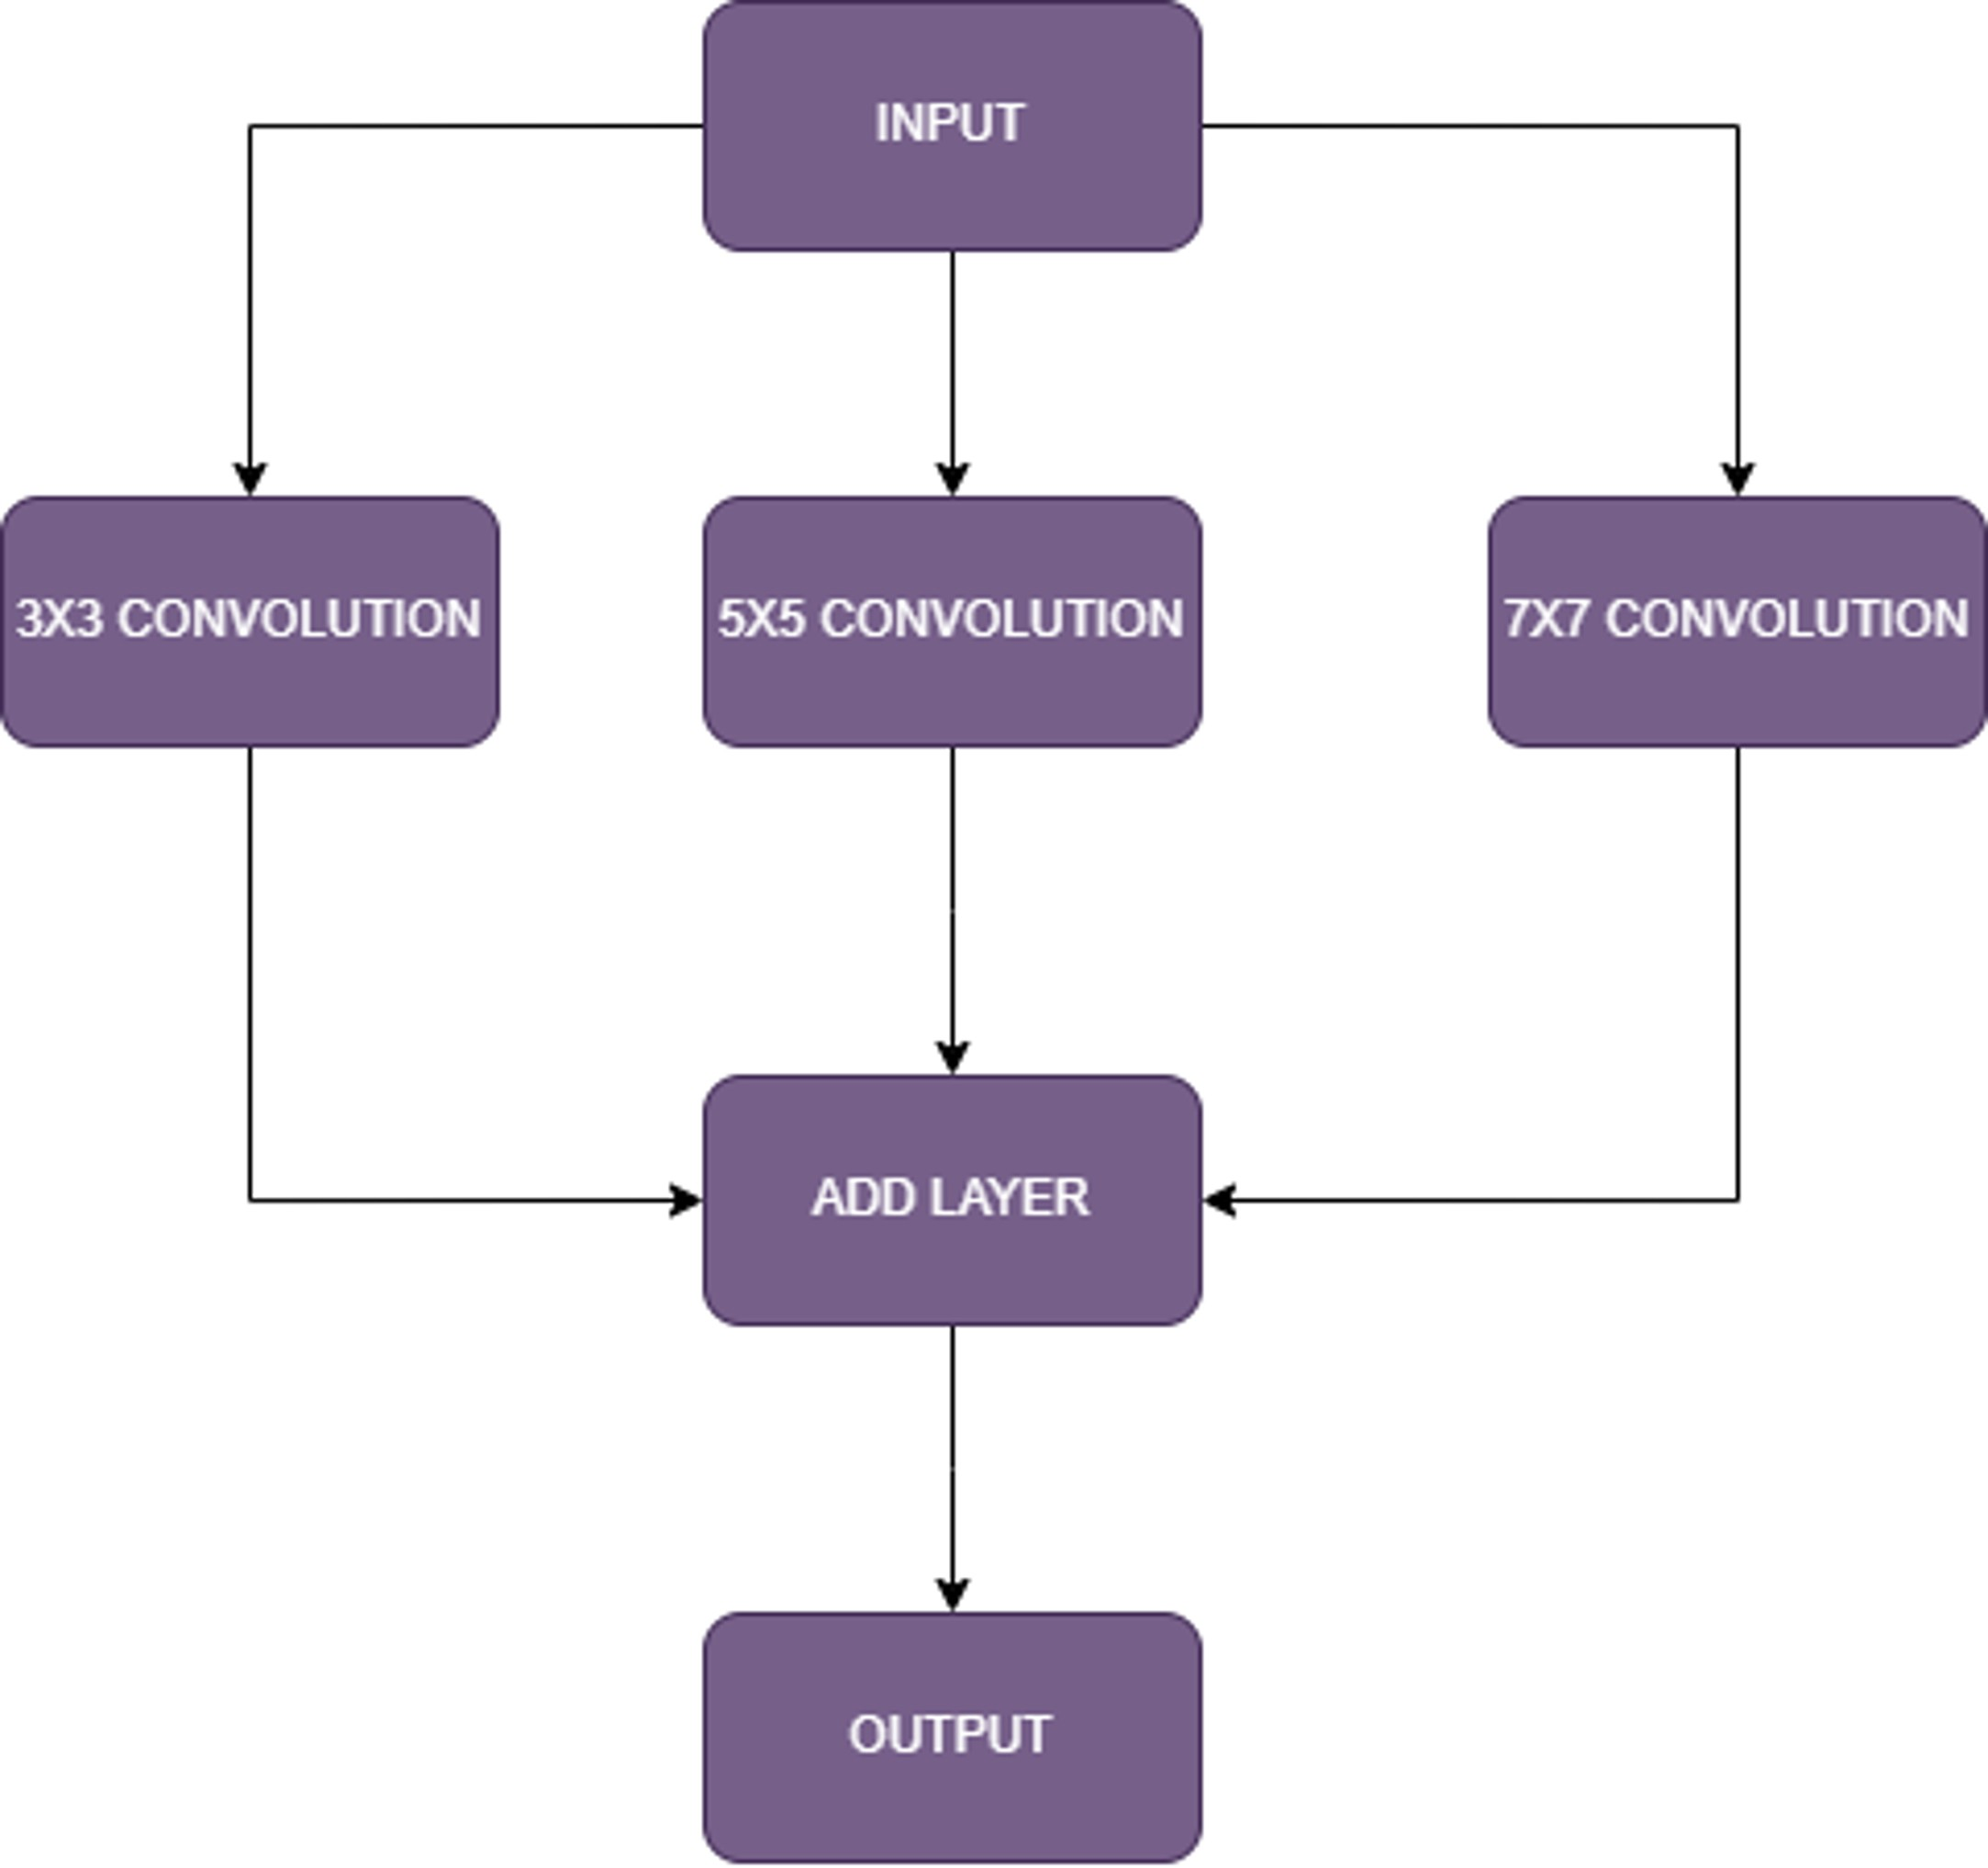
\includegraphics[width=0.68\textwidth,height=0.62\textheight,keepaspectratio]{paper_figures/inception_block.jpg}}{}
\caption{Proposed Inception(Add) block.}
\label{fig:inception}
\end{figure*}

\subsection{SkipConnection(Concat) block}
The skip block first applies a $7\times7$ convolution and batch normalization, and then concatenates the resulting feature maps with the original input:
\begin{equation}
Y=\operatorname{Concat}\left(X,F(X)\right).
\label{eq:concat}
\end{equation}
Unlike additive residual fusion, concatenation does not force the transformed and original representations to occupy the same feature channels. The input remains directly available to subsequent processing, while the newly learned features provide an additional representation. This design is inspired by the feature-reuse motivation of DenseNet \cite{huang2017}, but the present network uses it in two explicit blocks rather than adopting the full DenseNet connectivity pattern.

The cost is channel growth. Starting from 32 channels, the first skip block produces 96 channels, and the second produces 224 channels. This growth explains why concatenation is used selectively rather than inside the Inception cells.

\begin{figure*}[t]
\centering
\IfFileExists{paper_figures/skip_block.jpg}{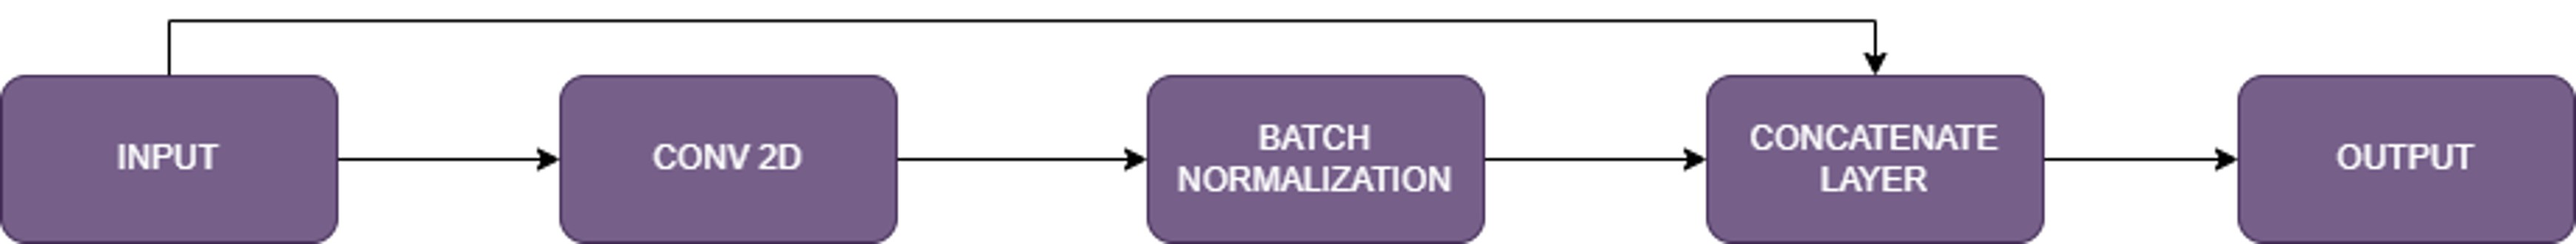
\includegraphics[width=0.68\textwidth,height=0.62\textheight,keepaspectratio]{paper_figures/skip_block.jpg}}{}
\caption{Proposed SkipConnection(Concat) block.}
\label{fig:skip}
\end{figure*}

\subsection{Classification head}
After the fourth max-pooling operation, global average pooling converts the $16\times16\times224$ representation into a 224-dimensional vector. Two fully connected layers with 512 and 128 units perform nonlinear classification before the final softmax layer. Dropout is used between the dense layers to reduce co-adaptation of features.

\begin{table*}[t]
\centering
\caption{Architecture of the implemented PlantDiseaseNet-Hybrid model.}
\label{tab:architecture}
\begin{tabular}{p{3.2cm}p{3.0cm}p{2.0cm}p{6.0cm}}
\toprule
Stage & Output & Parameters & Operation\\
\midrule
Input & $256\times256\times3$ & 0 & RGB input\\
Inception cell 1 & $256\times256\times16$ & 4,032 & $3\times3$, $5\times5$, $7\times7$ convolutions + Add\\
Batch normalization + Pool 1 & $128\times128\times16$ & 64 & Normalization + $2\times2$ max pooling\\
Inception cell 2 & $128\times128\times32$ & 42,592 & Multi-scale convolution + Add\\
Batch normalization + Pool 2 & $64\times64\times32$ & 128 & Normalization + $2\times2$ max pooling\\
Skip block 1 + Pool 3 & $32\times32\times96$ & 100,672 & $7\times7$ convolution + BN + Concat + pooling\\
Skip block 2 + Pool 4 & $16\times16\times224$ & 602,752 & $7\times7$ convolution + BN + Concat + pooling\\
GAP & 224 & 0 & Global average pooling\\
Dense 1 & 512 & 115,200 & ReLU\\
Dense 2 & 128 & 65,664 & ReLU\\
Output & 24 & 3,096 & Softmax\\
\bottomrule
\end{tabular}
\end{table*}

\subsection{Training protocol}
The primary model uses a batch size of 32 and a maximum of 60 training epochs. Adam is used as the optimizer with an initial learning rate of 0.001. Categorical cross-entropy is used for multi-class classification. The repository records cosine warmup annealing and early stopping with a patience of 12 for the proposed training configuration.

\begin{table}[t]
\centering
\caption{Primary training configuration.}
\label{tab:training}
\begin{tabular}{p{3.1cm}p{3.0cm}}
\toprule
Parameter & Setting\\
\midrule
Input size & $256\times256\times3$\\
Batch size & 32\\
Maximum epochs & 60\\
Optimizer & Adam\\
Learning rate & 0.001\\
Scheduler & Cosine warmup annealing\\
Early stopping & Patience 12\\
Loss & Categorical cross-entropy\\
\bottomrule
\end{tabular}
\end{table}

\subsection{Evaluation metrics}
Accuracy, precision, recall, F1-score, specificity, and ROC-AUC are retained as evaluation measures where the corresponding experiment provides the required prediction outputs. For multi-class evaluation, macro-averaged measures are preferred when class-wise behaviour is being compared, while weighted measures are used when class prevalence is relevant. ROC-AUC values are only reported when the underlying one-vs-rest probabilities and class labels support a valid calculation; undefined values are not replaced by artificial numerical values.

\section{Experimental Design}
The experiments are deliberately divided into four groups. The first group evaluates the proposed architecture on individual crop datasets and the combined dataset. The second group examines architecture substitutions on the combined dataset. The third group studies augmentation as a separate variable. The fourth group contains soybean experiments performed under a separate dataset setting.

\subsection{Primary experiments}
NB1, NB2, and NB3 apply the hybrid architecture to wheat, cotton, and PlantVillage data, respectively. The combined proposed model is represented by the executed \texttt{original-custom-hybrid} notebook. These experiments answer whether the architecture can operate across datasets with substantially different class counts and visual characteristics.

\subsection{Architecture ablation}
The ablation study compares four alternatives on the combined dataset: standard InceptionNet; a ResNet-style residual architecture; Inception with additive branch fusion; and skip-connection concatenation without the full hybrid arrangement. These are architecture ablations because the independent variable is the network design, while the dataset and task are held at the combined multi-crop setting. By contrast, simply changing a dataset is not itself an architecture ablation.

\section{Results}
\subsection{Primary results}
The crop-specific experiments show a substantial difference between datasets. Wheat and PlantVillage obtain accuracies of 97.81\% and 97.67\%, respectively, whereas the cotton experiment obtains 53.55\%. This spread is important: it prevents the conclusion that the architecture has uniform performance across all crops. Instead, the result indicates that the difficulty of the image distribution and class structure materially affects performance.

The combined 24-class proposed experiment reaches 95.91\%. Although this value is lower than the two strongest crop-specific experiments, the task is substantially broader because multiple crop and disease categories must be separated within one classifier. The combined result is therefore the principal multi-crop benchmark used for architecture comparison.

\subsection{Architecture ablation results}
The architecture comparison is summarized in Table~\ref{tab:ablation}. Standard Inception obtains 95.33\%, while the ResNet-style alternative reaches 96.04\%. The Inception+Add variant obtains 95.84\%, and the Skip+Concat variant obtains 95.67\%. The proposed combined architecture reaches 95.91\%.

\begin{table}[t]
\centering
\caption{Combined-dataset architecture ablation.}
\label{tab:ablation}
\begin{tabular}{p{3.4cm}c}
\toprule
Architecture & Accuracy (\%)\\
\midrule
Standard Inception & 95.33\\
ResNet-style & 96.04\\
Inception + Add & 95.84\\
Skip + Concat & 95.67\\
Full PlantDiseaseNet-Hybrid & 95.91\\
\bottomrule
\end{tabular}
\end{table}

The ablation results should not be interpreted as evidence that one fusion operation is universally superior. The isolated Inception+Add and Skip+Concat variants are close to the complete hybrid result, while the ResNet-style model is slightly higher in this particular experiment. The value of the proposed design is therefore architectural complementarity: additive multi-scale fusion controls channel growth early, whereas concatenative skip fusion preserves information later. The ablation establishes that neither component can be justified solely by an accuracy gain in isolation.

\subsection{Per-class and error analysis}
The repository stores confusion matrices, per-class metrics, ROC curves, and training histories for the primary logged experiments. These outputs should be used to identify which disease pairs are systematically confused, rather than relying only on the aggregate accuracy. In particular, the low cotton accuracy warrants inspection of its confusion matrix and class-wise precision/recall before any biological interpretation is made.

\subsection{Augmentation results and interpretation}
The augmentation experiments are presented as a dedicated study because they answer a different question from the architecture ablation: whether exposing the model to controlled appearance and geometric variability changes generalization. The repository contains several augmentation notebooks, including crop-specific and combined configurations, as well as a no-augmentation reference notebook. The stored notebooks do not provide a uniformly verifiable final test-metric record for every augmentation run. Therefore, this draft does not fabricate an augmentation ranking.

The intended final analysis is a controlled table with one row per augmentation condition and the same held-out test protocol across conditions. The table should report accuracy, precision, recall, F1-score, specificity, and, where valid, macro ROC-AUC. Training curves should be shown alongside the final metric table so that an apparent gain can be distinguished from overfitting or unstable optimization. This presentation is informed by Mhala et al. \cite{mhala2025}, while keeping the experimental conditions specific to this study.

\subsection{Soybean study}
Soybean experiments are reported separately because the ASDID setting is independent from the primary 24-class combined experiment. The repository contains six soybean notebooks. Executed outputs from the first two notebooks report 100\% accuracy, while other soybean notebooks do not currently provide a uniformly verifiable final metric in the stored output. These results should therefore be treated as a separate evaluation stream rather than combined numerically with the 24-class benchmark.

The soybean dataset is a field-oriented resource with eight disease/deficiency categories and healthy leaves, captured across multiple locations and seasons \cite{bevers2022,dryad2022}. Bevers et al. reported that augmentation could improve class parity in their soybean disease study \cite{bevers2022}. This makes the soybean section useful for examining behaviour under a different imaging setting, but it does not justify pooling soybean accuracy with the primary experiments.

\section{Computational Analysis}
The implemented hybrid model has 934,200 parameters when the complete layer and normalization parameters are counted from the supplied Keras architecture. An earlier draft contained a conflicting value of 933,426 parameters; that value should not be retained unless it can be reproduced from the exact final model object.

The architecture makes an explicit computational trade-off. Additive fusion prevents the three Inception branches from tripling the output depth. Concatenative skip fusion increases depth, but it does so only after the multi-scale extraction stages and preserves earlier features. This selective use of the two operations is the principal efficiency argument of the architecture.

\section{Discussion}
The most important observation from the primary experiments is not the highest accuracy but the variation between datasets. The same hybrid design obtains high accuracy on wheat and PlantVillage while substantially lower accuracy on cotton. This indicates that model architecture alone does not determine the difficulty of disease recognition. Class overlap, sample distribution, visual variability, image quality, and dataset construction can all influence the outcome.

The combined experiment provides the most appropriate setting for the architectural comparison because all ablation variants are evaluated on the same multi-crop task. The full hybrid result of 95.91\% is competitive with the isolated alternatives, but the ablation does not show a dramatic numerical advantage. Consequently, the scientific claim should be framed around the complementary design rationale and controlled comparison rather than an unsupported claim of universal superiority.

The Inception(Add) block is motivated by representation efficiency. Parallel kernels provide multiple receptive fields, while addition keeps the output depth fixed. This is attractive at the high-resolution early stages of the network, where channel expansion is expensive. The skip concatenation block serves a different purpose: it retains earlier information so that later layers do not have to reconstruct it. The architecture therefore follows a stage-specific fusion strategy rather than applying one operation everywhere.

Augmentation should be interpreted similarly. A transformation is useful only if it represents plausible variation in the target deployment environment. Excessive or unrealistic transformations can increase intra-class variation without adding useful information. For this reason, the final augmentation section should report the exact transformation ranges and compare matched training conditions. The present repository evidence supports describing the transformation families, but not yet a complete numerical ranking across all augmentation notebooks.

\section{Limitations}
Several limitations should be acknowledged. First, the primary datasets are not equivalent in difficulty or class composition, so cross-dataset accuracy comparisons should not be treated as a ranking of dataset quality. Second, the repository contains multiple experimental generations; some notebooks are duplicated, incomplete, or exploratory. The organized research branch therefore distinguishes executed evidence from notebooks retained for provenance.

Third, the soybean experiments use a separate dataset and should not be interpreted as an additional 24-class benchmark. Fourth, high accuracy on controlled or curated leaf datasets does not automatically establish field robustness. Finally, the current augmentation notebooks do not provide a complete, uniformly verifiable final metric set for every condition; the final manuscript should populate those values only after the corresponding stored outputs have been checked.

\section{Conclusion}
This study presented PlantDiseaseNet-Hybrid, a hybrid CNN that deliberately assigns different fusion operations to different stages of feature extraction. Inception branches with $3\times3$, $5\times5$, and $7\times7$ kernels are fused by addition to control channel growth, while later transformed features are concatenated with their inputs to preserve and reuse information.

The executed primary experiments demonstrate that the architecture can operate across wheat, cotton, PlantVillage, and a combined multi-crop setting, although performance varies substantially by dataset. The architecture ablation shows that the complete hybrid design is competitive with simpler alternatives, while also making clear that its value should be described as complementary feature fusion rather than as a universally superior operation.

The study is deliberately structured so that primary evaluation, augmentation analysis, architecture ablation, and soybean evaluation remain separate. This separation is essential for a defensible scientific interpretation because changing the dataset, architecture, and augmentation policy simultaneously would make causal attribution impossible. The final manuscript should add only those augmentation and soybean metrics that can be traced directly to executed repository outputs.

\section*{Data and Code Availability}
The research repository contains the executed notebooks, stored result logs, architecture figures, and manuscript source. Public dataset sources should be cited in their original scholarly or archival form rather than through a secondary Kaggle mirror where an authoritative source is available.

\section*{Declaration of Competing Interest}
The authors declare no competing interests.

\section*{Funding}
No external funding was received for this study.

\bibliographystyle{cas-model2-names}
\begin{thebibliography}{00}
\bibitem{mohanty2016} S. P. Mohanty, D. P. Hughes, M. Salathé, Using deep learning for image-based plant disease detection, Frontiers in Plant Science 7 (2016) 1419. doi:10.3389/fpls.2016.01419.
\bibitem{szegedy2015} C. Szegedy, W. Liu, Y. Jia, P. Sermanet, S. Reed, D. Anguelov, D. Erhan, V. Vanhoucke, A. Rabinovich, Going deeper with convolutions, in: Proceedings of the IEEE Conference on Computer Vision and Pattern Recognition, 2015, pp. 1--9. doi:10.1109/CVPR.2015.7298594.
\bibitem{he2016} K. He, X. Zhang, S. Ren, J. Sun, Deep residual learning for image recognition, in: Proceedings of the IEEE Conference on Computer Vision and Pattern Recognition, 2016, pp. 770--778. doi:10.1109/CVPR.2016.90.
\bibitem{huang2017} G. Huang, Z. Liu, L. van der Maaten, K. Q. Weinberger, Densely connected convolutional networks, in: Proceedings of the IEEE Conference on Computer Vision and Pattern Recognition, 2017, pp. 4700--4708.
\bibitem{mhala2025} P. Mhala, A. Bilandani, S. Sharma, Enhancing crop productivity with fine-tuned deep convolution neural network for potato leaf disease detection, Expert Systems with Applications 267 (2025) 126066. doi:10.1016/j.eswa.2024.126066.
\bibitem{bevers2022} N. Bevers, E. J. Sikora, N. B. Hardy, Soybean disease identification using original field images and transfer learning with convolutional neural networks, Computers and Electronics in Agriculture 203 (2022) 107449. doi:10.1016/j.compag.2022.107449.
\bibitem{dryad2022} N. Bevers, E. J. Sikora, N. B. Hardy, Pictures of diseased soybean leaves by category captured in field and with controlled backgrounds: Auburn soybean disease image dataset (ASDID), Dryad Dataset, 2022. doi:10.5061/dryad.41ns1rnj3.
\end{thebibliography}
\end{document}
